\section{解析几何}{
  不容小觑且难以理解的部分,加油.

  \subsection{关于向量}{
    在空间解析几何部分不会引入过多有关线性代数的知识(比如向量空间).定理与定义将会互相交织.

    注:本章中的向量默认为三维向量.

    \subsubsection{关于向量的基本概念}{
      有以下概念:
      \begin{itemize}
        \item 数乘:$\lambda \vec{\alpha}$,即$\lambda$倍长度的$\vec{\alpha}$,当$\lambda > 0$时,方向与原向量相同.当$\lambda < 0$时,方向相反.数乘前后向量的起点一致.
        \item 取模:$|\lambda\vec{\alpha}| = |\lambda||\vec{\alpha}|$,前一个“$||$”为绝对值,后一个“$||$”为取模.最后得出的结果为$|\lambda\vec{\alpha}|$的长度.
        \item 单位化:$|\cfrac{\vec{\alpha}}{|\vec{\alpha}|}| = 1$,即将一个向量除以他的长度得到的是单位向量(长度为1的向量)
        \item 在三维标准正交坐标系中存在三个单位向量:$\vec{i},\vec{j},\vec{k}$.他们互相垂直,长度为1.坐标系中任意一点$(x,y,z)$都可以表示为一个向量$\vec{r},\vec{r} = x\vec{i} + y\vec{j} + z\vec{k}$.
        \item 设$\vec{a} = (ax,ay,az),\vec{b} = (bx,by,bz)$.则:$\vec{a} \pm \vec{b} = (ax \pm bx,ay \pm by,az \pm bz)$、$\lambda\vec{a} = (\lambda ax,\lambda ay,\lambda az)$.其中$ax,ay,az,bx,by,bz$称为分量.
        \item 平行:$\vec{b} = \lambda\vec{a},\cfrac{ax}{bx} = \cfrac{ay}{by} = \cfrac{az}{bz}$即:对应分量之比相同.
        \item 向量长度(取模)公式:$\vec{r} = (x,y,z),|\vec{r}| = \sqrt{x^2 + y^2 + z^2}$.注:对于任意维度的向量,取模都是各分量平方和开根号.
        \item 两点之间距离公式:$A:(x_1,y_1,z_1),B:(x_2,y_2,z_2),|\vec{AB}| = \sqrt{(x_1 - x_2)^2 + (y_1 -y_2)^2 + (z_1 - z_2)^2}$.注:在任意维度中,两点之间的距离公式都是对应分量作差的平方和开根号.
        \item {
              两向量夹角:(取锐角)设$\vec{a} = (a_1, a_2, a_3),\vec{b} = (b_1,b_2,b_3)$,设夹角为$\theta$,则:$\cos\theta = \cfrac{|a_1b_1 + a_2b_2 + a_3b_3|}{\sqrt{a_1^2 + a_2^2 + a_3^2}\sqrt{b_1^2 + b_2^2 + b_3^2}}$

              有以下几种情况:
              \begin{enumerate}
                \item 垂直:$a_1b_1 + a_2b_2 + a_3b_3 = 0$
                \item 平行:$\cfrac{a_1}{b_1} = \cfrac{a_2}{b_2} = \cfrac{a_3}{b_3}$
              \end{enumerate}

              求两直线夹角也同理.
              }
      \end{itemize}
    }%关于向量的基本概念结尾

    \subsubsection{方向角与方向余弦}{
      \begin{center}
        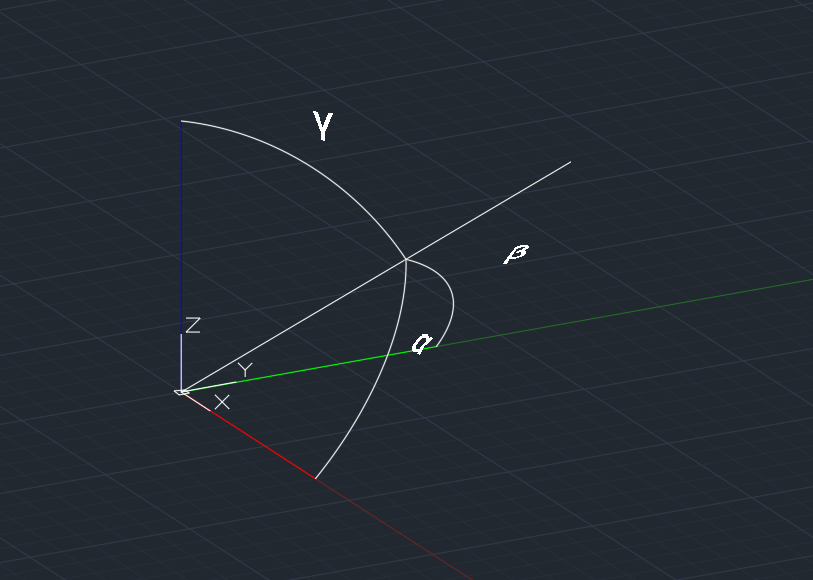
\includegraphics[scale = 0.5]{resources/directionAngle.png}
      \end{center}

      $\vec{OM} = \vec{r} = (x,y,z)$

      $\cos\alpha = \cfrac{x}{|\vec{OM}|} = \cfrac{x}{|\vec{r}|}$

      $\cos\beta = \cfrac{y}{|\vec{OM}|} = \cfrac{y}{|\vec{r}|}$

      $\cos\gamma = \cfrac{z}{|\vec{OM}|} = \cfrac{z}{|\vec{r}|}$

      其中$\alpha,\beta,\gamma$称为$\vec{OM}$的方向角.

      有恒等式:$\cos^2\alpha + \cos^2\beta + \cos^2\gamma = 1$

      方向余弦是指在解析几何里,一个向量的三个方向余弦分别是这向量与三个坐标轴之间的角度的余弦.两个向量之间的方向余弦指的是这两个向量之间的角度的余弦.在此处指的是前者,也就是:$\cos\alpha,\cos\beta,\cos\gamma$.

      将方向余弦作为三个分量,即:$(\cos\alpha,\cos\beta,\cos\gamma) = (\cfrac{x}{|\vec{r}|}, \cfrac{y}{|\vec{r}|}, \cfrac{z}{|\vec{r}|}) = \cfrac{1}{|\vec{r}|}\vec{r} = e_r$

      其中$e_r$是个单位向量,表示以向量$\vec{r}$的方向余弦为坐标的向量.

    }%方向角与方向余弦结尾

    \subsubsection{向量投影}{
      \begin{center}
        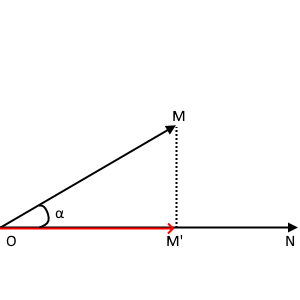
\includegraphics{resources/vector_axis_projection.png}
      \end{center}

      直接写出来:
      \begin{enumerate}
        \item $\projection{u}\vec{a} = |\vec{a}|\cdot\cos\alpha$
        \item $\projection{u}(\vec{a} + \vec{b}) = \projection{u}\vec{a} + \projection{u}\vec{b}$
        \item $\projection{u}\lambda\vec{a} = \lambda\projection{u}a$
      \end{enumerate}

      $u$:任意轴\qquad$\vec{a}$:向量\qquad$\projection{u}$:投影到u轴

    }%向量投影结尾

    \subsubsection{数量积/点乘}{
      点乘算出来的是数

      $\vec{a} \cdot \vec{b} = |a|\cdot|b|\cdot\cos\theta = |a|\cdot\projection{a}b = |b|\cdot\projection{b}a$

      $\theta$:夹角\\

      \indent点乘有以下性质:
      \begin{enumerate}
        \item $\vec{a}\cdot\vec{a} = |a|\cdot|a|\cdot\cos0 = |a|^2$
        \item $\vec{a}\cdot\vec{b} = 0,\theta = 90\degree,\vec{a} \perp \vec{b}$\qquad 即:$\vec{a}\cdot\vec{b} = 0 \Leftrightarrow \vec{a} \perp \vec{b}$
        \item $\vec{a}\cdot\vec{b} = \vec{b}\cdot\vec{a}$
        \item $(\vec{a}+\vec{b})\cdot\vec{c} = \vec{a}\cdot\vec{c} + \vec{b}\cdot\vec{c}$
        \item $(\lambda\vec{a})\cdot\vec{b} = \lambda(\vec{a}\cdot\vec{b})$
        \item $\vec{a} = (a_x,a_y,a_z),\vec{b} = (b_x,b_y,b_z),\vec{a}\cdot\vec{b} = a_xb_x + a_yb_y + a_zb_z$
        \item $\cos\theta = \cfrac{\vec{a}\cdot\vec{b}}{|\vec{a}|\cdot|\vec{b}|} = \cfrac{a_xb_x + a_yb_y + a_zb_z}{\sqrt{a_x^2 + a_y^2 + a_z^2}\cdot\sqrt{b_x^2 + b_y^2 + b_z^2}}$
      \end{enumerate}

    }%数量积/点乘结尾

    \subsubsection{向量积/叉乘}{
      叉乘算出来的是向量,这个向量垂直于其他两个向量.右手法则:食指为$\vec{a}$,中指为$\vec{b}$,拇指为$\vec{c}$

      $\vec{a}\times\vec{b} = \vec{c}$

      其中:$\vec{c}\perp\vec{a},\vec{c}\perp\vec{b}$\\

      \indent有以下性质:
      \begin{itemize}
        \item $\vec{a}\times\vec{a} = 0$
        \item 有非零向量$\vec{a},\vec{b},\vec{a}\times\vec{b} = 0\ \Rightarrow \vec{a} // \vec{b}$.即:$\vec{a} // \vec{b} \Leftrightarrow \vec{a} \times \vec{b} = 0$
        \item $\vec{b}\times\vec{a} = -\vec{b}\times\vec{a}$
        \item $(\vec{a} + \vec{b})\times\vec{c} = \vec{a} \times \vec{c} + \vec{b} \times \vec{c}$
        \item $(\lambda\vec{a})\times\vec{b} = \vec{a} \times (\lambda\vec{b}) = \lambda(\vec{a}\times\vec{b})$
      \end{itemize}

      有两种计算方法:

      首先,设$\vec{a} = (a_1,a_2,a_3),\vec{b} = (b_1,b_2,b_3)$,并将结果向量记作$\vec{s}$:

      \begin{itemize}
        \item {
              坐标形式:

              $$
                \vec{s}
                =
                \vec{a}\times\vec{b}
                =
                \begin{bmatrix}
                  s_1 \\
                  s_2 \\
                  s_3
                \end{bmatrix}
                =
                \begin{bmatrix}
                  a_2b_3 - a_3b_2 \\
                  a_3b_1 - a_1b_3 \\
                  a_1b_2 - a_2b_1
                \end{bmatrix}
              $$
              }
        \item {
              行列式形式:

              $$
                \vec{s}
                =
                \vec{a}\times\vec{b}
                =
                \left|\begin{array}{ccc}
                  \vec{i} & \vec{j} & \vec{k} \\
                  a_1     & a_2     & a_3     \\
                  b_1     & b_2     & b_3
                \end{array}\right|
              $$
              }
      \end{itemize}
    }%向量积/叉乘结尾

  }%关于向量结尾

  \subsection{关于圆}{

    \subsubsection{圆的方程}{
      \begin{center}
        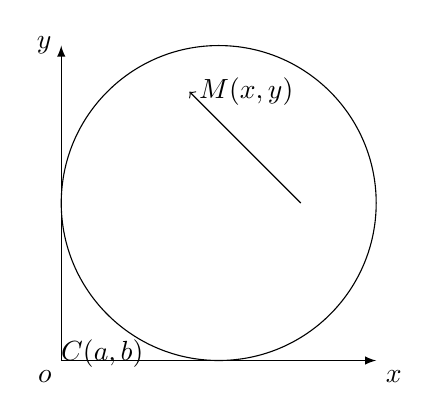
\begin{tikzpicture}
          \draw[-latex] (0,0) node[below left]{$o$} -- (4,0) node[below right]{$x$};
          \draw[-latex] (0,0) -- (0,4) node[left]{$y$};
          \draw  (2,2) circle (2);
          \tikzPlaceDot{(2,2) node [above right]{$C(a,b)$}};
          \draw[->] (2,2) -- ({2 - sqrt(2)},{2 + sqrt(2)}) node[right]{$M(x,y)$};
        \end{tikzpicture}
      \end{center}

      \begin{itemize}
        \item {
              圆的标准方程 : $(x - a)^2 + (y - b)^2 = r^2$

              由圆的定义可知,$\absoluteValue{\vec{CM}} = r$,因此 : $$
                \sqrt{(x - a)^2 + (y - b)^2} = r
              $$
              即,以$C(a,b)$为圆心,$r$为半径的圆的方程为 : $$
                (x - a)^2 + (y - b)^2 = r^2
              $$
              }
        \item {
              圆的一般方程 : $x^2 + y^2 + Dx + Ey + F = 0$

              将标准方程展开可得以上形式,反过来,也可以将以上形式配方,得到 : $$
                \bigCase{x + \cfrac{D}{2}}^2 + \bigCase{y + \cfrac{E}{2}}^2 = \cfrac{D^2 + E^2 - 4F}{4}
              $$

              \begin{enumerate}
                \item $D^2 + E^2 - 4F$称为圆方程的判别式,暂时把他记作$\alpha$吧(非正式用法,只在本章有效).
                \item 当$\alpha > 0$时,把一般方程和圆的标准方程比较,可以看出此一般方程表示以$\bigCase{-\cfrac{D}{2},-\cfrac{E}{2}}$为圆心,半径为$\cfrac{1}{2}\sqrt{D^2 + E^2 - 4F}$的圆.
                \item 当$\alpha = 0$时,方程只有一个实数解-也就是说方程只表示唯一的一个点$\bigCase{-\cfrac{D}{2},-\cfrac{E}{2}}$.
                \item 当$\alpha < 0$时,方程没有实数解,此时方程没有图形.
              \end{enumerate}

              因从,当$\alpha > 0$时,此种方程形式就叫做圆的一般方程,这种形式有以下特点 :
              \begin{enumerate}
                \item $x^2$与$y^2$的系数相同且不为0.
                \item 不含$xy$项.
                \item $D^2 + E^2 - 4F > 0$.
              \end{enumerate}
              }
      \end{itemize}
    }%圆的方程结尾

    \subsubsection{圆的切线方程}{
      已知$M(x_0,y_0)$为圆$x^2 + y^2 = r^2$上的一点,求过点$M$的圆$C$的切线$l$的方程 :

      因为$M$是$l$与圆$C$的切点,所以过$M$的半径$OM$与$l$垂直,即$\vec{OM}=\begin{bmatrix}
          x_0 \\ y_0
        \end{bmatrix}$是$l$的法向量,于是可得切线$l$的点法向式方程 : $$
        x_0(x - x_0) + y_0(y - y_0) = 0
      $$
      整理后可得 : $$
        x_0x + y_0y = x_0^2 + y_0^2
      $$
      又因为$M$在$C$上,因此$x_0^2 + y_0^2 = r^2$,最终得到切线的方程为 : $$
        x_0x + y_0y = r^2
      $$
    }%圆的切线方程结尾

  }%关于圆结尾

  \subsection{关于椭圆}{

    \subsubsection{椭圆的一般方程}{
      \begin{center}
        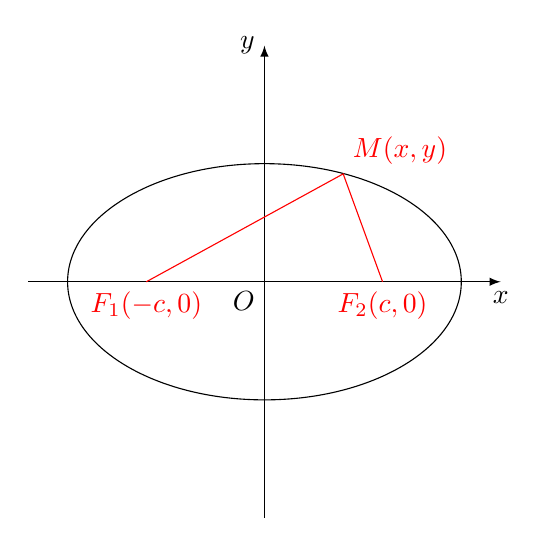
\begin{tikzpicture}
          \draw[-latex] (-3,0) -- node[below left]{$O$} (3,0)node [below]{$x$};
          \draw[-latex] (0,-3) -- (0,3)node [left]{$y$};
          \draw (0,0) ellipse (2.5 and 1.5);
          \draw[red] (1.5,0) node[below]{$F_2(c,0)$} -- (1,1.37) node[above right]{$M(x,y)$} -- (-1.5,0) node[below]{$F_1(-c,0)$};
        \end{tikzpicture}
      \end{center}

      将平面内到两个定点$F_1,F_2$的距离之和等于常数$2a$的点的轨迹叫做椭圆.这两个定点叫做椭圆$EC$的焦点,两个焦点的距离$\absoluteValue{F_1F_2}$称为椭圆的焦距.

      根据定义,建系建立方程,设焦距为$2c$,$F_1,F_2$的坐标分别为$(-c,0),(c,0)$.设$M(x,y)$是椭圆上任意一点,点$M$到两焦点的距离和等于$2a(a>c>0)$. : $$
        \absoluteValue{MF_1} + \absoluteValue{MF_2} = \sqrt{(x + c)^2 + y^2} + \sqrt{(x - c)^2 + y^2} = 2a
      $$
      将第二项移到右边,两边平方再整理,得 : $$
        a^2 - cx = a\sqrt{(x - c)^2 + y^2}
      $$
      两边再平方,经过整理,得 : $$
        (a^2 - c^2)x^2 + a^2y^2 = a^2(a^2 - c^2)
      $$
      由于$a^2 - c^2 > 0$,设$吧^2 = a^2 - c^2$ : $$
        b^2x^2 + a^2y^2 = a^2b^2
      $$
      即 : $$
        \cfrac{x^2}{a^2} + \cfrac{y^2}{b^2} = 1(a>b>0)
      $$
      同理,如果焦点在y轴上,那么方程就是 : $$
        \cfrac{y^2}{a^2} + \cfrac{x^2}{b^2} = 1(a > b > 0)
      $$

      这其实是一种很漂亮的形式 :

      \begin{center}
        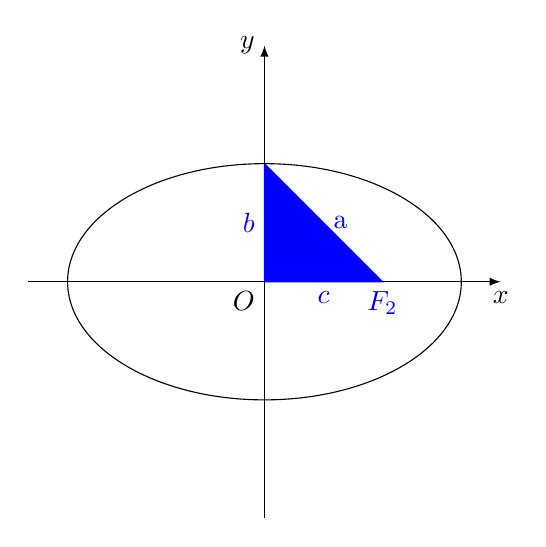
\begin{tikzpicture}
          \draw[-latex] (-3,0) -- node[below left]{$O$} (3,0)node [below]{$x$};
          \draw[-latex] (0,-3) -- (0,3)node [left]{$y$};
          \draw (0,0) ellipse (2.5 and 1.5);
          \filldraw[blue] (1.5,0) node[below]{$F_2$} -- node[below]{$c$} (0,0) -- node[left]{$b$}(0,1.5) -- node[right]{a} cycle;
        \end{tikzpicture}
        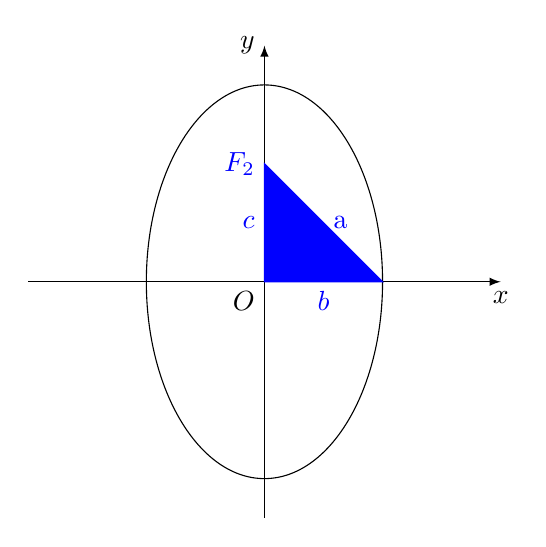
\begin{tikzpicture}
          \draw[-latex] (-3,0) -- node[below left]{$O$} (3,0)node [below]{$x$};
          \draw[-latex] (0,-3) -- (0,3)node [left]{$y$};
          \draw (0,0) ellipse (1.5 and 2.5);
          \filldraw[blue] (0,1.5) node[left]{$F_2$} -- node[left]{$c$} (0,0) -- node[below]{$b$}(1.5,0) -- node[right]{a} cycle;
        \end{tikzpicture}
      \end{center}

      这就是椭圆的标准方程.
    }%椭圆的一般方程结尾

  }%关于椭圆结尾

  \subsection{关于空间平面}{

    \subsubsection{空间平面公式}{
      法线向量与平面垂直.\\

      \indent空间平面有以下表示方法:
      \begin{itemize}
        \item {
              点法式:知道一点与法线向量.

              设一点$M_0:(x_0,y_0,z_0)$,法线向量:$\vec{n} = (A,B,C)$

              设$M(x,y,z),\vec{M_0M}=(x - x_0,y - y_0,z - z_0),\vec{n} \cdot \vec{M_0M} = 0$

              平面的点法式方程为:$A(x - x_0) + B(y - y_0) + C(z - z_0) = 0$
              }
        \item {
              一般式:三点确定一个向量.以实例演示:

              设$M_1(2,-1,4),M_2(-1,3,-2),M_3(0,2,3)$代入:

              $Ax + By + Cz + D = 0$

              $$
                \begin{cases}
                  2A - B + 4C = -D \\
                  -A + 3B -2C = -D \\
                  2B + 3C = -D
                \end{cases}
              $$

              也有$Ax + By + Cz + (-Ay_0 - By_0 - Cz_0) = 0$

              (由点法式推出)\\

              \indent有以下情况:
              \begin{enumerate}
                \item $D = 0,Ax + By + Cz = 0$:平面过原点.
                \item $A = 0,By + Cz + D = 0$:法线垂直与$x$轴且平面平行于$x$轴,类似情况同理
                \item $A = B = 0,CZ + D = 0$:平面过$z = -\cfrac{D}{C}$,平行于$xy$轴.
              \end{enumerate}
              }
        \item 截距式:$\cfrac{x}{a} + \cfrac{y}{b} + \cfrac{z}{c} = 1$
      \end{itemize}
    }%关于空间平面结尾

    \subsubsection{求两平面夹角}{
      其实是求两平面法线的夹角(取锐角)

      因此只要设两平面法线向量为$n_1(A_1,B_1,C_1),n_2(A_2,B_2,C_2)$,然后套向量夹角公式就行了.

      其中$\theta = (\widehat{n_1\ n_2})$或$(\widehat{-n_1\ n_2}) = (\pi - (\widehat{n_1\ n_2}))$

      其中当向量平行时意味着平面重合(因为取的是锐角)、
    }%求两平面夹角结尾

    \subsubsection{点到平面距离公式}{
      设点$P_0(x_0,y_0,z_0),Ax + By + Cz + D = 0$

      $d = \cfrac{|Ax_0 + By_0 + Cz_0 + D|}{\sqrt{A^2 + B^2 + C^2}}$
    }%点到平面距离公式结尾

    \subsubsection{直线与平面夹角}{
      指的是直线与法线的夹角

      设与直线同方向的向量$L_1(M,N,P)$,夹角为$\theta$

      $\sin\theta = \cfrac{|AM + BN + CP|}{\sqrt{A^2 + B^2 + C^2}\sqrt{M^2 + N^2 + P^2}}$\\

      \indent有以下几种情况:
      \begin{enumerate}
        \item 直线垂直于平面: $\cfrac{A}{M} = \cfrac{B}{N} = \cfrac{C}{P}$
        \item 直线平行于平面: $AM + BN + CP = 0$
      \end{enumerate}
    }%直线与平面夹角结尾

  }%空间平面及其方程结尾

  \subsection{关于空间直线}{

    \subsubsection{空间直线及其方程}{
      有以下三种形式:

      \begin{enumerate}
        \item {
              一般方程:(即两平面的交线)

              $$
                \begin{cases}
                  A_1x + B_1y + C_1Z + D_1 = 0 \\
                  A_2x + B_2y + C_2z + D_2 = 0
                \end{cases}
              $$
              }
        \item {
              对称式方程:

              设点$M(x,y,z),M_0(x_0,y_0,z_0)$是直线$L$上的任意两点,那么存在向量$\vec{M_0M}$与直线$L$的方向向量$\vec{s}$平行.因此两向量的对应坐标成比例.$(\vec{M_0M} = (x - x_0, y - y_0, z - z_0), \vec{s} = (m,n,p))$,因此得出:

              $\cfrac{x - x_0}{m} = \cfrac{y - y_0}{n} = \cfrac{z - z_0}{p} = t$
              }
        \item {
              参数式:将对称式变形

              $$
                \begin{cases}
                  x = x_0 + mt \\
                  y = y_0 + nt \\
                  z = z_0 + pt
                \end{cases}
              $$
              }
      \end{enumerate}
    }%空间直线及其方程结尾

    \subsubsection{平面束}{
      平面束即形成一条直线的所有面

      $$
        \begin{cases}
          A_1x + B_1y + C_1z + D_1 = 0 \\
          A_2x + B_2y + C_2z + D_2 = 0
        \end{cases}
      $$

      其中$A_1,B_1,C_1$与$A_2,B_2,C_2$不成比例.即:$A_1x + B_1y + C_1z + D_1 + \lambda(A_2x + B_2y + C_2z + D_2) = 0, (\lambda \in \mathRealNumberCollection)$
    }%平面束结尾

  }%关于空间直线结尾

  \subsection{关于空间曲线}{

    \subsubsection{空间曲线及其方程}{
      有以下两种形式:

      \begin{enumerate}
        \item {
              一般式:(两曲面的交线)

              $$
                \begin{cases}
                  F(x,y,z) = 0 \\
                  G(x,y,z) = 0
                \end{cases}
              $$
              }
        \item {
              参数方程:(将曲线上的动点的坐标表示为参数t的函数)

              $$
                \begin{cases}
                  x = x(t) \\
                  y = y(t) \\
                  z = z(t)
                \end{cases}
              $$
              }
      \end{enumerate}
    }%空间曲线及其方程结尾

    \subsubsection{参数方程与一般方程的互化}{
      这两者之间的互化往往会用到一些特殊的技巧,比如诱导公式.

      举例 : 设一个圆的参数方程为 : $$
        \begin{cases}
          x = -1 + \cos \theta \\
          y = 3 + \sin \theta
        \end{cases}
        \mbox{($\theta$是参数)}
      $$

      仅列出以下解法 :
      \begin{enumerate}
        \item {
              利用平方关系$\cos^2\theta + \sin^2\theta = 1$,先将原方程整理一下 : $$
                \begin{cases}
                  \cos\theta = x + 1 \\
                  \sin\theta = y - 3
                \end{cases}
              $$
              代入得 : $$
                (x + 1)^2 + (y - 3)^2 = 1
              $$
              }
        \item {
              类比圆的参数方程形式 : $$
                \begin{cases}
                  x = x_0 + r\cos\alpha \\
                  y = y_0 + r\sin\alpha
                \end{cases}
              $$

              可知圆心为$(-1,3)$,半径$r = 1$,所以普通方程为 : $$
                (x + 1)^2 + (y - 3)^2 = 1
              $$
              }
      \end{enumerate}

      关键在于如何利用一般情况下的公式的结构,而且需要明确参数和角度的区别(因为往往$\theta$是被看作参数而非角度).
    }%参数方程与一般方程的互化结尾

    \subsubsection{常见参数方程}{
      以下都是二维参数方程.

      \begin{itemize}
        \item {
              直线 :
              \begin{itemize}
                \item 点斜式 : 过$(x_0,y_0)$,斜率为$m$的直线 : $\begin{cases}
                          x = x_0 + y \\
                          y = y_0 + mt
                        \end{cases}$
                \item 点向式 : 过$(x_0,y_0)$,方向向量为$(u,v)$的直线 : $\begin{cases}
                          x = x_0 + ut \\
                          y = y_0 + vt
                        \end{cases}$
              \end{itemize}
              }
        \item 圆 : $\begin{cases}
                  x = r\cos t \\
                  y = r\sin t
                \end{cases}$
        \item 椭圆 : $\begin{cases}
                  x = a\cos t \\
                  y = b\sin t
                \end{cases}$
        \item 双曲线 : $\begin{cases}
                  x = a\sec t \\
                  y = b\tan t
                \end{cases}$
        \item 抛物线 : $\begin{cases}
                  x = 2ct \\
                  y = t^2
                \end{cases}$
        \item 螺线 : $\begin{cases}
                  x = t\cos lt \\
                  y = t\sin lt
                \end{cases}$
        \item 摆线 : $\begin{cases}
                  x = r \cdot (t - \sin t) \\
                  y = r \cdot (1 - \cos t)
                \end{cases}$
      \end{itemize}

      注 : 上文中的$a,b,c,h,k,l,m,p,r,x_0,y_0,u,v$为已知数,$t$都是参数,$x,y$为一般方程下的变量.
    }%常见参数方程结尾

    \subsubsection{空间曲线在坐标系面上的投影}{

      设空间曲线c的一般方程为:

      $$
        \begin{cases}
          F(x,y,z) = 0 \\
          G(x,y,z) = 0
        \end{cases}
      $$

      消去其中一个变量,(比如z),求在xoy上的投影,得到方程:

      $$
        \begin{cases}
          F(x,y) = 0 \\
          z = 0
        \end{cases}
      $$
    }%空间曲线在坐标系面上的投影结尾

    \subsubsection{空间曲线的切线及法平面}{
      先写出空间曲线的切线方程 :

      $$
        \begin{cases}
          x = \varphi(t) \\
          y = \Phi(t)    \\
          z = \omega(t)
        \end{cases}
      $$

      其中 $t \in [\alpha,\beta]$,设三个函数都可导且不同时为0.

      则切向量$\vec{T} = \begin{bmatrix}
          \varphi\derivative(t_0) & \Phi\derivative(t_0) & \omega\derivative(t_0)
        \end{bmatrix}$

      切线方程为 : $\cfrac{x - x_0}{\varphi\derivative(t_0)} = \cfrac{y - y_0}{\Phi\derivative(y_0)} = \cfrac{z - z_0}{\omega\derivative(t_0)}$

      则法平面的点法式方程为 : $\varphi\derivative(t_0)(x - x_0) + \Phi\derivative(t_0)(y - y_0) + \omega\derivative(z - z_0) = 0$
    }%空间曲线的切线及法平面

    \subsubsection{空间曲线的切平面及法线}{
      有两种情况 :

      \begin{enumerate}
        \item {
              $F(x,y,z) = 0$(即隐函数)

              则切平面的方程为:$F\derivative_x(x_0,y_0,z_0)(x - x_0) + F\derivative_y(x_0,y_0,z_0)(y - y_0) + F\derivative_z(x_0,y_0,z_0)(z - z_0) = 0$

              法线的方程为 : $\cfrac{x - x_0}{F\derivative_x(x_0,y_0,z_0)} = \cfrac{y - y_0}{F\derivative_y(x_0,y_0,z_0)} = \cfrac{z - z_0}{F\derivative_z(x_0,y_0,z_0)}$
              }
        \item {
              $z = \defFunction{x,y}$,只需让$F = \defFunction{x,y} - z$,然后套公式1.

              切平面解析式为 : $f\derivative_x(x_0,y_0)(x - x_0) + f\derivative_y(x_0,y_0)(y - y_0) - (z - z_0) = 0$
              }
      \end{enumerate}
    }%空间曲线的切平面及法线

  }%关于空间曲线结尾

  \subsection{关于空间曲面}{

    \subsubsection{空间曲面及其方程}{
      有非常多种曲面,都给他列出来:

      \begin{itemize}
        \item {
              旋转曲面:由二次曲线绕某一坐标轴旋转形成.

              \begin{itemize}
                \item {
                      设YOZ平面上有曲线$\defFunction{y,z} = 0$:

                      \begin{itemize}
                        \item 绕z轴旋转,曲面表达式为:$\defFunction{\pm\sqrt{x^2 + y^2},z} = 0$
                        \item 绕y轴旋转,曲面表达式为:$\defFunction{y,\pm\sqrt{x^2 + z^2}} = 0$
                      \end{itemize}
                      }
                \item {
                      设XOY平面上有曲线$\defFunction{x,y} = 0$:

                      \begin{itemize}
                        \item 绕x轴旋转,曲面表达式为:$\defFunction{x,\pm\sqrt{y^2 + z^2}} = 0$
                        \item 绕y轴旋转,曲面表达式为:$\defFunction{\pm\sqrt{x^2 + z^2},y} = 0$
                      \end{itemize}
                      }
                \item {
                      设XOZ平面上有曲线$\defFunction{x,z} = 0$:

                      \begin{itemize}
                        \item 绕x轴旋转,曲面表达式为:$\defFunction{x,\pm\sqrt{y^2 + z^2}} = 0$
                        \item 绕z轴旋转,曲面表达式为:$\defFunction{\pm\sqrt{x^2 + y^2},z} = 0$
                      \end{itemize}
                      }
              \end{itemize}
              }
        \item {
              二次曲面:

              二次曲面有以下12种:
              \begin{itemize}
                \item {
                      椭球面:

                      在直角坐标系中的方程为:

                      $\cfrac{x^2}{a^2} + \cfrac{y^2}{b^2} + \cfrac{z^2}{c^2} = 1$

                      其中a和b是赤道半径(沿着x和y轴),c是极半径,(沿着z轴).这三个数都是固定的正实数,决定了椭球的形状.

                      如果三个半径都是相等的,那么就是一个球;如果有两个半径是相等的,则是一个类球面.

                      \begin{itemize}
                        \item $a = b = c$:球
                        \item $a = b > c$:扁球面
                        \item $a = b < c$:长球面
                        \item $a \neq b,b \neq c,c \neq a$:不等边椭球(三条边都不相等)
                      \end{itemize}

                      点(a,0,0)、(0,b,0)和(0,0,c)都在曲面上.从原点到这三个点的线段,称为椭球的半主轴.它们与椭圆的半长轴和半短轴相对应.

                      体积公式为:$\cfrac{4}{3}\pi abc$.

                      注意,当三个半径都相等时,这个公式便化为球的体积;两个半径相等时,便化为扁球面或长球面的体积.
                      }
                \item {
                      抛物面:

                      例:$y^2 - 2x = 0 / F(x,y) = 0$,参数中缺少z,因此母线平行于z轴
                      }
                \item {
                      椭圆抛物面:

                      椭圆抛物面在直角坐标系中的方程为:$z = \cfrac{x^2}{a^2} + \cfrac{y^2}{b^2}$
                      }
                \item {
                      双曲抛物面:

                      双曲抛物面在直角坐标系中的方程为:$z = \cfrac{x^2}{a^2} - \cfrac{y^2}{b^2}$
                      }
                \item {
                      单叶双曲面:

                      单叶双曲面在直角坐标系中的方程为:$\cfrac{x^2}{a^2} + \cfrac{y^2}{b^2} - \cfrac{z^2}{c^2} = 1$

                      当a = b时双曲面就会变得比较圆
                      }
                \item {
                      双叶双曲面:

                      双叶抛物面在直角坐标系中的方程为:$\cfrac{x^2}{a^2} + \cfrac{y^2}{b^2} - \cfrac{z^2}{c^2} = -1$

                      当a = b时双曲面就会变得比较圆
                      }
                \item {
                      类球面:

                      类球面是一种二次曲面.二维的椭圆有两个主轴,称为长轴与短轴.在三维空间里,将一个椭圆绕着其任何一主轴旋转,则可得到一个类球面.

                      \begin{itemize}
                        \item 假若,这旋转主轴是长轴,则这个类球面为长球面.例如,英式足球里所用的橄榄球是长球形状.
                        \item 假若,这旋转主轴是短轴,则这个类球面为扁球面.例如,地球在北极与南极稍微有点扁平,在赤道又有点凸涨.所以,地球是扁球形状.
                        \item  假若,生成的椭圆是圆圈,则这个类球面为完全对称的圆球面.
                      \end{itemize}

                      用另一种方法来描述,类球面是一种椭球面.而椭球面的公式已经给出,其中a与b分别是椭球面在x轴与y轴的赤道半径,c是椭球面在z轴的极半径,这三个正实数的半径决定了椭球面的形状.以z轴为旋转轴的类球面a = b,他的方程为:

                      $\cfrac{x^2 + y^2}{a^2} + \cfrac{z^2}{c^2} = 1$

                      \begin{itemize}
                        \item 如果三个半径都相等,则此椭球面是圆球面$(a = c)$
                        \item 如果类球面的赤道半径小于极半径,则这是类球面中的长球面.$(a < c)$
                        \item 如果类球面的赤道半径大于极半径,则这是类球面中的扁球面.$(a > c)$
                      \end{itemize}
                      }
                \item {
                      球面:

                      在空间解析几何中,球心为$(x_0,y_0,z_0)$,半径为r的球面是满足以下方程的所有点的轨迹:

                      $(x - x_0)^2 + (y - y_0)^2 + (z - z_0)^2 = r^2$

                      当球心在原点上:$x^2 + y^2 + z^2 = r^2$

                      可化作三元二次方程:$Ax^2 + Ay^2 + Az^2 + Bx + Cy + Dz + G = 0$(平方项系数相同)

                      其中$D^2 + E^2 + F^2 > 4AG$.

                      当满足以上两点时可逆推出一个三元二次方程是否为一个球面

                      (当$D^2 + E^2 + F^2 = 4AG$时是一个点)
                      }
                \item {
                      椭圆锥面(二次锥面):

                      椭圆锥面在直角坐标系中的方程为:$\cfrac{x^2}{a^2} + \cfrac{y^2}{b^2} - \cfrac{z^2}{c^2} = 0$

                      当a = b时就会变成圆锥面.
                      }
                \item {
                      椭圆柱面:

                      椭圆柱面在直角坐标系中的方程为:$\cfrac{x^2}{a^2} + \cfrac{y^2}{b^2} = 1$

                      当a = b时就会变成圆柱面.
                      }
                \item {
                      双曲柱面:

                      双曲柱面在直角坐标系中的方程为:$\cfrac{x^2}{a^2} - \cfrac{y^2}{b^2} = 1$
                      }
                \item {
                      抛物柱面:

                      抛物柱面在直角坐标系中的方程为:$x^2 + 2ay = 0$
                      }
              \end{itemize}
              }
      \end{itemize}
    }%空间曲面及其方程结尾

    \subsubsection{伸缩法}{
      注:伸缩法不是放缩法!

      举例:有$x^2 + y^2 = 1$,沿着y轴伸缩两倍,则伸缩后的方程为:$x^2 + \cfrac{y^2}{4} = 1$.

      也就是说:沿着n轴伸缩,就对变量n进行替换.

      伸缩t倍,就把原变量替换成$\cfrac{n}{t}$
    }%伸缩法结尾
  }%关于空间曲面结尾

 }%解析几何结尾